\documentclass[11pt]{article} % Font size
%\usepackage[utf8]{inputenc}
%\usepackage{graphicx}
%\graphicspath{{Figures/}{./}}
%\usepackage[slovak]{babel}
%\usepackage{amsmath}
%%%%%%%%%%%%%%%%%%%%%%%%%%%%%%%%%%%%%%%%%
% Wenneker Assignment
% Structure Specification File
% Version 2.0 (12/1/2019)
%
% This template originates from:
% http://www.LaTeXTemplates.com
%
% Authors:
% Vel (vel@LaTeXTemplates.com)
% Frits Wenneker
%
% License:
% CC BY-NC-SA 3.0 (http://creativecommons.org/licenses/by-nc-sa/3.0/)
% 
%%%%%%%%%%%%%%%%%%%%%%%%%%%%%%%%%%%%%%%%%

%----------------------------------------------------------------------------------------
%	PACKAGES AND OTHER DOCUMENT CONFIGURATIONS
%----------------------------------------------------------------------------------------

\usepackage{amsmath, amsfonts, amsthm} % Math packages

\usepackage{listings} % Code listings, with syntax highlighting

\usepackage[slovak]{babel} % English language hyphenation

\usepackage{graphicx} % Required for inserting images
\graphicspath{{Figures/}{./}} % Specifies where to look for included images (trailing slash required)

\usepackage{booktabs} % Required for better horizontal rules in tables

\usepackage{caption}
\usepackage{subcaption}

\numberwithin{equation}{section} % Number equations within sections (i.e. 1.1, 1.2, 2.1, 2.2 instead of 1, 2, 3, 4)
\numberwithin{figure}{section} % Number figures within sections (i.e. 1.1, 1.2, 2.1, 2.2 instead of 1, 2, 3, 4)
\numberwithin{table}{section} % Number tables within sections (i.e. 1.1, 1.2, 2.1, 2.2 instead of 1, 2, 3, 4)

\setlength\parindent{0pt} % Removes all indentation from paragraphs

\usepackage{enumitem} % Required for list customisation
\setlist{noitemsep} % No spacing between list items

%----------------------------------------------------------------------------------------
%	DOCUMENT MARGINS
%----------------------------------------------------------------------------------------

\usepackage{geometry} % Required for adjusting page dimensions and margins

\geometry{
	paper=a4paper, % Paper size, change to letterpaper for US letter size
	top=2cm, % Top margin
	bottom=2cm, % Bottom margin
	left=2cm, % Left margin
	right=2cm, % Right margin
	headheight=0.75cm, % Header height
	footskip=1.5cm, % Space from the bottom margin to the baseline of the footer
	headsep=0.75cm, % Space from the top margin to the baseline of the header
	%showframe, % Uncomment to show how the type block is set on the page
}

%----------------------------------------------------------------------------------------
%	FONTS
%----------------------------------------------------------------------------------------

\usepackage[utf8]{inputenc} % Required for inputting international characters
\usepackage[T1]{fontenc} % Use 8-bit encoding

\usepackage{fourier} % Use the Adobe Utopia font for the document

%----------------------------------------------------------------------------------------
%	SECTION TITLES
%----------------------------------------------------------------------------------------

\usepackage{sectsty} % Allows customising section commands

\sectionfont{\vspace{6pt}\centering\normalfont\scshape} % \section{} styling
\subsectionfont{\normalfont\bfseries} % \subsection{} styling
\subsubsectionfont{\normalfont\itshape} % \subsubsection{} styling
\paragraphfont{\normalfont\scshape} % \paragraph{} styling

%----------------------------------------------------------------------------------------
%	HEADERS AND FOOTERS
%----------------------------------------------------------------------------------------

\usepackage{scrlayer-scrpage} % Required for customising headers and footers

\ohead*{} % Right header
\ihead*{} % Left header
\chead*{} % Centre header

\ofoot*{} % Right footer
\ifoot*{} % Left footer
\cfoot*{\pagemark} % Centre footer
 % Include the file specifying the document structure and custom commands

%----------------------------------------------------------------------------------------
%	TITLE SECTION
%----------------------------------------------------------------------------------------

\title{	
	\normalfont\normalsize
	\textsc{Slovenská technická univerzita v Bratislave, fakulta elektrotechniky a informatiky}\\ % Your university, school and/or department name(s)
	\vspace{25pt} % Whitespace
	%\rule{\linewidth}{0.5pt}\\ % Thin top horizontal rule
	\vspace{20pt} % Whitespace
	\vspace{20pt} % Whitespace
	\vspace{20pt} % Whitespace
	\vspace{20pt} % Whitespace
	\vspace{20pt} % Whitespace
	\vspace{20pt} % Whitespace
	\vspace{20pt} % Whitespace
	\vspace{20pt} % Whitespace
		\vspace{20pt} % Whitespace
	\vspace{20pt} % Whitespace
	\huge Farmakokinetika a farmakodynamika inzulínu\\ % The assignment title
	\vspace{12pt} % Whitespace
	\normalsize Biokybernetika, zadanie č.2
	\vspace{20pt} % Whitespace
	\vspace{20pt} % Whitespace
	\vspace{20pt} % Whitespace
		\vspace{20pt} % Whitespace
	\vspace{20pt} % Whitespace
		\vspace{20pt} % Whitespace
	\vspace{20pt} % Whitespace
		\vspace{20pt} % Whitespace
	\vspace{20pt} % Whitespace
	\vspace{20pt} % Whitespace
	\vspace{20pt} % Whitespace
		\vspace{20pt} % Whitespace
	\vspace{20pt} % Whitespace
	%\rule{\linewidth}{2pt}\\ % Thick bottom horizontal rule
	\vspace{12pt} % Whitespace
}

\author{\LARGE Lukáš Šníder} % Your name

\date{november 2020}
%\date{\normalsize\today} 

\begin{document}

\maketitle % Print the title
\thispagestyle{empty}
\clearpage
\setcounter{page}{1}
\pagenumbering{arabic} 
%----------------------------------------------------------------------------------------
%	FIGURE EXAMPLE
%----------------------------------------------------------------------------------------

\section{Zostavenie simulačnej schémy podsystému pre vstrebávanie inzulínu}

\subsection{Opis modelu podsystému vstrebávania inzulínu}

Tento podsystém je reprezentovaný nasledovnými rovnicami:
%\begin{align*}
\begin{eqnarray}
	\dot{S_1}(t) &=& -\left(\frac{1}{T_I}\right) S_1(t) + v(t) \\ 
	\dot{S_2}(t) &=& -\left(\frac{1}{T_I}\right)S_2(t) + \left(\frac{1}{T_I}\right)S_1(t) \\
	\dot{I}(t) &=& -{k_I}I(t) + \left(\frac{1}{T_I}\right)\left(\frac{1}{V_I}\right)S_2(t) 
\end{eqnarray}

Vstupom je rýchlosť podávania inzulínu \textit{v(t)} $[\mu U/kg/min]$ do podkožia, parametrami sú: \textbf{$T_I$ $[min]$}, čo je časová konštanta podsystému, \textbf{$k_I$ $[l/min]$} je rýchlosť samovoľného ubúdania inzulínu a \textbf{$V_I$ $[ml/kg]$} je objem na kilogram hmotnosti. Výstupom je koncentrácia inzulínu v krvi \textit{I(t)}.

\subsection{Zobrazenie dát reprezentujúcich farmakokinetiku a ich príprava}

Farmakokinetické dáta inzulínu sme dostali v csv súbore v jednotkách [pmol/l], sú zobrazené na obrázku \ref{fig:pk_data}, kedže ale koncetráciu inzulínu modelujeme v $[\mu U/ml]$ a platí 1 U = 6000 pmol, musíme ich premeniť podľa vzorca:
\begin{equation}
1 \hspace{1mm} [pmol/l] = 1/6 \hspace{1mm} [\mu U/ml] 
\end{equation}

Dáta po tejto premene jednotiek je možné vidieť na obrázku \ref{fig:pk_data_2}.

\begin{figure} % [h] forces the figure to be output where it is defined in %the code (it suppresses floating)
\begin{subfigure}{.5\textwidth}
	\centering
	
	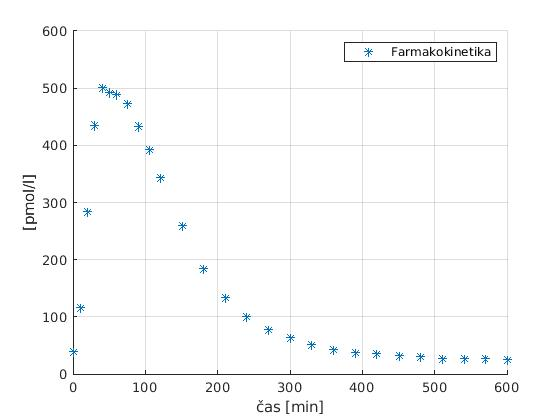
\includegraphics[width=1.0\linewidth]{pk_data.jpg} % Example image
	\caption{Vstupné dáta farmakokinetiky}
	\label{fig:pk_data}
\end{subfigure}
\begin{subfigure}{.5\textwidth}
	\centering
	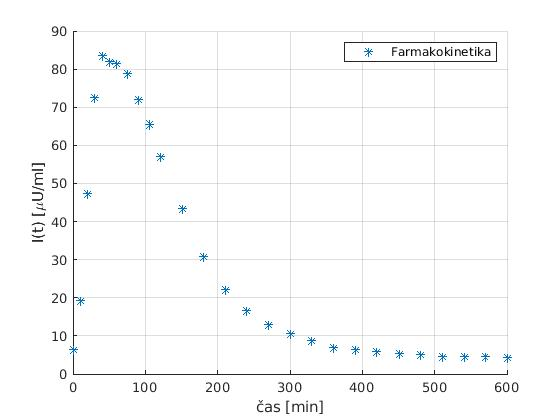
\includegraphics[width=1.0\linewidth]{pk_data_2.jpg} % Example image
	\caption{Upravené vstupné dáta farmakokinetiky}
	\label{fig:pk_data_2}
\end{subfigure}
\caption{FK dáta}
\end{figure} 
S takto pripravenými dátami sme už pripravený vykonať vzorovú simuláciu.

\newpage

\subsection{Vzorová simulácia}

\begin{figure}[h]
	\centering
	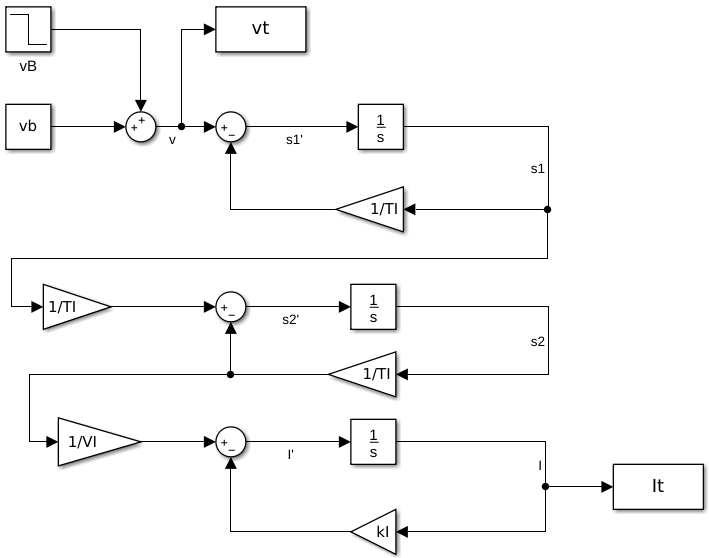
\includegraphics[width=0.9\columnwidth]{podsystem_vstrebavania.png} 
	\caption{Schéma podsystému vstrebávania inzulínu.}
	\label{fig:schema}
\end{figure}

Ako sme už spomenuli vstupom do modelu je rýchlosť podávania inzulínu $v(t)$, tá pozostáva z dvoch rýchlostí a to sú bazálna rýchlosť ${v_b}$ a rýchlosť podávania bolusu $v_B$, v našom prípade to bolo: 

\begin{equation}
v_B(t) = 40000 \hspace{1mm} [\mu U/kg/min] 
\end{equation}
\begin{equation}
v_b(t) = 281.218 \hspace{1mm} [\mu U/kg/min]
\end{equation}

Podávanie bolusu $v_B$ simulujeme tak, že počas prvej periódy vzorkovania $T_S$, pre $T_S$ = 5 $[min]$, privádzame na vstup signál uvedenej veľkosti $v_B(t)$ = 40000 $[\mu U/kg/min]$ a pre zvyšný čas je to $v_B(t)$ = 0, veľkosť bazálnej rýchlosti $v_b(t)$ = 281.218 $[\mu U/kg/min]$ máme vypočítanú zo záznamov inzulínovej pumpy subjektu a v simulácií sme ju definovali ako konštantnú vstupnú hodnotu. Na nasledujúcom obrázku \ref{fig:v_podavania_I} je zobrazený priebeh tejto rýchlosti.

\begin{figure}[h] 
	\centering
	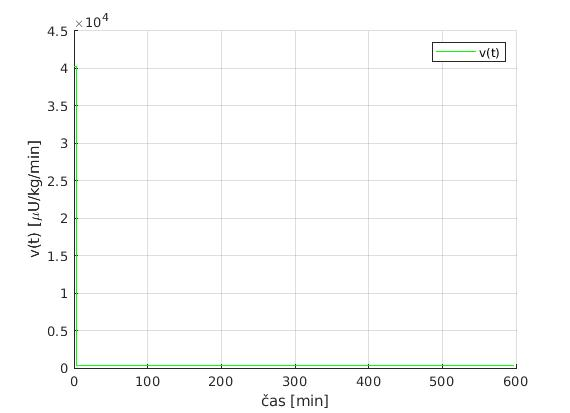
\includegraphics[width=0.6\columnwidth]{rychlost_podavania.jpg} 
	\caption{Priebeh rýchlosti podávania inzulínu.}
	\label{fig:v_podavania_I}
\end{figure}

Keďže bazálna koncentrácia nameraných dát je 6.5 $[\mu U/kg/min]$, túto hodnotu sme zadefinovali ako počiačnú pre koncentráciu inzulínu.

Hodnoty parametrov tohto modelu, ktoré použijeme v našej vzorovej simulácií sú takéto:
\\

$T_I = 44,55 [min] $, \hspace{5mm}
$k_I = 0,1645 [l/min]$, \hspace{5mm}
$V_I = 138,8 [dl/kg]$
\\

Schéma, ktorú sme vytvorili, sa nachádza na obrázku \ref{fig:schema}. Samotnú simmuláciu sme nastavili na 600 sekúnd s periódou vzorkovania 1 minúta. Výsledný priebeh vzorovej simulácie je na obrázku \ref{fig:sim_vystup}.


\begin{figure}[h]
	\centering
	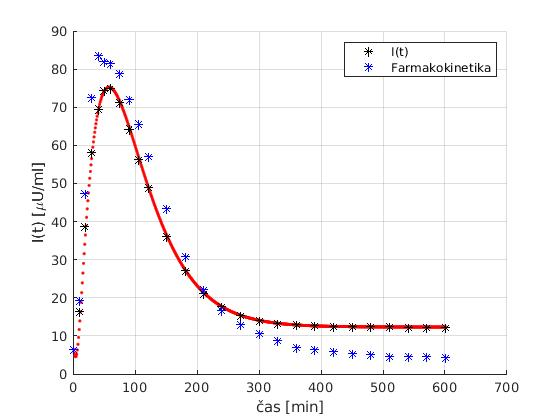
\includegraphics[width=0.6\columnwidth]{vzorova_simulacia_vystup.jpg} 
	\caption{Koncentrácia podávania inzulínu vzorovej simulácie.}
	\label{fig:sim_vystup}
\end{figure}

\newpage
\subsection{Identifikácia parametrov} \label{subsec:ids1}
Budeme idetifikovať parametre modelu podsystém vstrebávania inzulínu, teda
\begin{itemize}
\item $T_I$ $[min]$ - časová konštanta podsystému,
\item $k_I$ $[l/min]$ - rýchlosť samovoľného ubúdania inzulínu
\item $V_I$ $[dl/kg]$ - objem na kilogram hmotnosti
\end{itemize}

Pri identifikáci sme sa rozhodli použiť genetický algoritmus. Pre účely tejto úlohy si z hľadaných parametrov vyskladáme chromozóny jedincov, ktoré budú vystupovať v evolúcií nášho genetického algoritmu, takže každý jedinec bude pozostávať z troch génov $T_I$, $k_I$, $V_I$. 

Na začiatku je dôležité vhodne si zadefinovať stavový priestor prehľadávania, t.j. horné a dolné ohraničenie pre jednotlivé parametre. Pri ich nesprávnom nastavení sa môže stať, že sa nám nepodarí nájsť dostatočne dobré riešenie, po niekoľkých testoch sme sa dostali k nasledovným ohraničeniam: 
\[ 10 < T_I < 70, \hspace{3mm} 0.01 < k_I < 1, \hspace{3mm} 20 < V_I < 200\] 
V rámci samotného algoritmu sme sa snažili zvoliť stredne veľký selektívny tlak a stredne veľkú diverziu, takže sme vyberali do ďalšej generácie 10\% najlepších jedincov z aktuálnej populácie a pre zvyšok sme volili mutácie na úrovni 20\%. Dĺžku evolúcie sme nastavili na 50 generácií, ale vzhľadom na vývoje účelových fitness funkcií, ktoré sme pozorovali možno úsúdiť, že stačilo aj 20 alebo 30 generácií, ako možno pozorovať na obrázku \ref{fig:moja_evolucia}

\begin{figure}
	\centering
	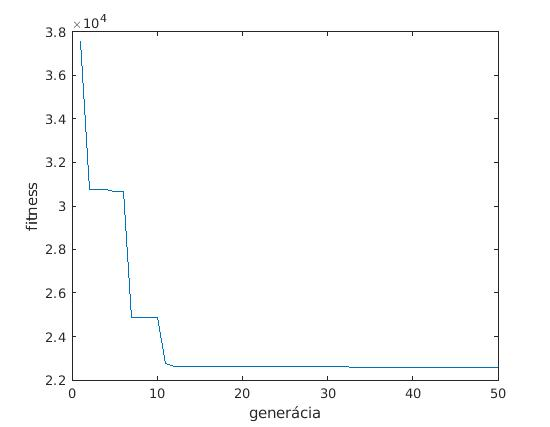
\includegraphics[width=0.7\columnwidth]{priebeh_evolucie.jpg} 
	\caption{Evolúcia účelovej funkcie pre naše riešenie.}
	\label{fig:moja_evolucia}
\end{figure}

Pri tvorbe samotnej účelovej funkcie sme vychádzali z učebného textu a vytvorili nasledovnú:

\begin{equation}
 min \hspace{5mm} \| y - \hat{y}(\theta_I) \|^2 \hspace{2mm}  + \hspace{2mm}  \gamma (V_{In} - V_I) \hspace{2mm}  + \hspace{2mm} \delta \sum(I(t) max(0, \arctan(t-200)))
\end{equation} 

kde prvá časť \[\| y - \hat{y}(\theta_I) \|^2\] je prebraná z učebného textu, a je to rozdiel štvorcov nameraných hodnôt farmakokinetiky $y$ a simulovaných hodnôt $\hat{y}$, ktoré boli simulované na základe parametrov $\theta_I = [T_I \hspace{1mm} k_I \hspace{1mm} V_I]$, druhá časť \[\gamma (V_{In} - V_I)\] bola rovnako inšpirovaná učebným textom, kde $V_{In}$ je normálna hodnota distribučného inzulínu, v našom prípade $100 [dl/kg]$, $\gamma$ je váhovací koeficient, $\gamma = 5 \times 10^{-4}$.

V tretej časti \[\delta \sum(I(t) max(0, \arctan(t-200)))\] sa snažíme o zlepšenie idenfikácia po 200-tej minúte simulácie.
Prenásobujeme tu vektory koncentrácie inzulínu $I(t)$ a vektor $max(0, \arctan(t-200) $, ktorý vynuluje hodnoty menšie ako 200 a hodnoty vyššie ako 200 sa budú pohybovať v intervale $(0,\pi/2)$, presnejšie v $\langle 1,5658;1,5691  \rangle$, takže čím budú hodnoty $I(t)$ vyššie so stúpajúcim časom simulácie $t$, tým to bude zvyšovať hodnotu celej účelovej funkcie. Tým sme sa snažili penalizovať pomalé klesanie v druhej časti simulácie (po 200-tej minúte). $\delta$ je váhovací koeficient tejto časti, $\delta = 0,01$. 

Nakoniec sa nám týmto postupom podarilo identifikovať nasledujúce parametre:
\begin{itemize}
\item $T_I = 41,8746 \hspace{1mm}[min]$ 
\item $k_I = 0,1459 \hspace{1mm}[l/min]$ 
\item $V_I = 147,7954 \hspace{1mm}[dl/kg]$ 
\end{itemize}

Na obrázku \ref{fig:vlastna_simulacia_vystup} je priebeh koncentrácie inzulínu po aplikovaní našich parametrov do simulácie.
 
\begin{figure}[h]
	\centering
	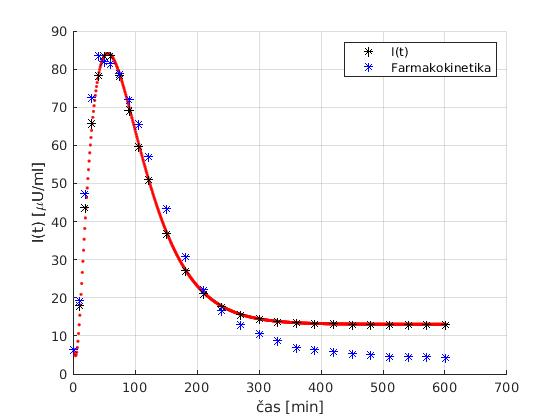
\includegraphics[width=0.7\columnwidth]{vlastna_simulacia_vystup.jpg} 
	\caption{Koncentrácia podávania inzulínu identifikovanými parametrami.}
	\label{fig:vlastna_simulacia_vystup}
\end{figure}

%\vspace{5mm}
%\[\]
%fit(j) = sum(abs(intDataFK/6 - It).^2) + lambda*((VIn - VI)^2) + gamma*(sum(It.*max(0,atan(tout-200))));... 

%\clearpage
%\newpage
\vspace{10mm}

\section{Pridanie podsystému vstrebávania inzulínu k Bergmanovmu minimálnemu modelu}

\subsection{Opis modifikácie Bergmanovho minimálneho modelu}

Bergmanov minimálny model, s ktorým budeme v tejto časti pracovať, je tvorený týmito diferenciálnymi rovnicami:
%\begin{align*}
\begin{eqnarray}
	\dot{X}(t) &=& -p_2X(t) + p_2 S_I (I(t)-I_b) \label{eq:bmm1} \\ 
	\dot{G}(t) &=& -(S_G + X(t))G(t) + S_G G_B + \left(\frac{1}{V_G}\right)Ra(t) \label{eq:bmm2} 
\end{eqnarray}
Pre účely priameho dávkovania glukózy do krvi, do Bergmanovho minimálneho modelu pribudol člen $\left(\frac{1}{V_G}\right)Ra(t)$, v ktorom je $Ra(t)$ $[mg/kg/min]$ je rýchlosť prísunu glukózy do krvi a parameter ${V_G}$ je objem na kilogram hmotnosti, do ktorého sa distribuuje glokóza. 

Vstupmi teda sú koncentrácia inzulínu v plazme $I(t)$ $[\mu U/ml]$ a práve spomenutá rýchlosť prísunu glukózy do krvi $Ra(t)$ $[mg/kg/min]$.

Hľadanými parametrami sú index inzulínovej citlivosti $S_I$ $[ml/\mu U/min]$ a obrátená hodnota časovej konštanty $p_2$ $[1/min]$

 
%jeho vstupom je  . Parametre sú index inzulínovej citlivosti $S_I$ $[ml/\mu U/min]$ a obrátená hodnota časovej konštanty $p_2$ $[1/min]$

\subsection{Zobrazenie dát reprezentujúcich farmakodynamiku a ich príprava}

Dáta farmakodynamiky máme podobne ako farmakokinetiku k dispozícií v csv súbore, môžme ich vidieť na obrázku \ref{fig:pd_data_1}. 
Opäť si ich budeme musieť premeniť, keďže tieto dáta vstupujú do modelu ako $Ra(t)$ $[mg/kg/min]$, zatiaľ čo v súbore sú v jednotkách $[mg/min]$, takže ich predelíme hmotnosťou. Tá sa v učebnom texte priamo nenachádza, ale vieme ju odvodiť z údaja o podanom boluse ($0,2 [U/kg]$) a celkovom boluse ($12,92 [U]$), z toho vyplýva, že hmotnosť subjektu je $12,92 / 0,2 = 64,6 [kg]$.

Takže farmakodynamické dáta budeme deliť hodnotou 64,6 $[kg]$ a takto premenené dáta môžme vidieť na obrázku \ref{fig:pd_data_2}.%kde sú tieto dáta

%\begin{figure}[h]
%	\centering
%	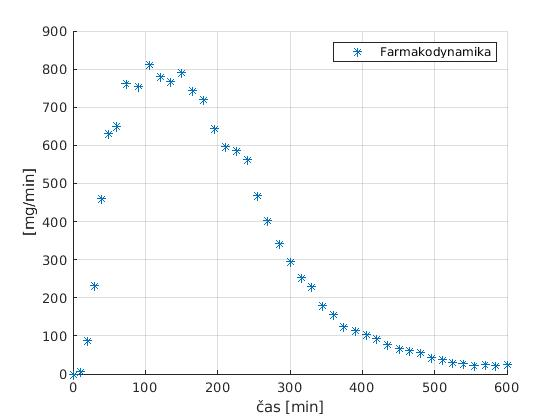
\includegraphics[width=0.7\columnwidth]{pd_data.jpg} 
%	\caption{Vstupné dáta farmakodynamiky}
%	\label{fig:pd_data.jpg}
%\end{figure}

\begin{figure} % [h] forces the figure to be output where it is defined in %the code (it suppresses floating)
\begin{subfigure}{.5\textwidth}
	\centering
	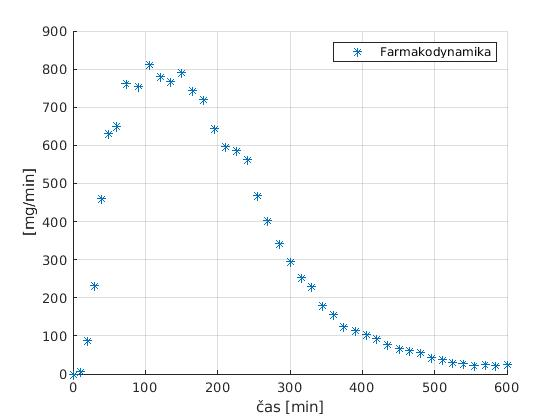
\includegraphics[width=1.0\linewidth]{pd_data.jpg} % Example image
	\caption{Vstupné dáta farmakodynamiky}
	\label{fig:pd_data_1}
\end{subfigure}
\begin{subfigure}{.5\textwidth}
	\centering
	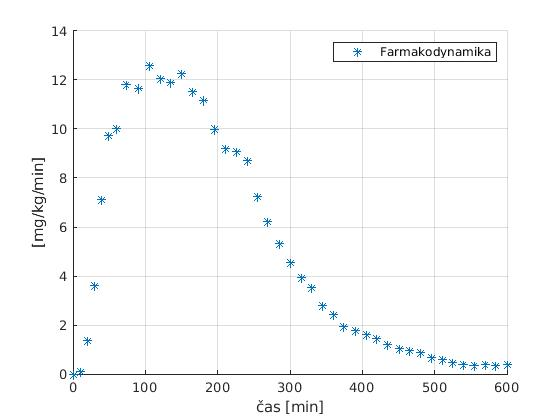
\includegraphics[width=1.0\linewidth]{pd_data_2.jpg} % Example image
	\caption{Upravené vstupné dáta farmakodynamiky}
	\label{fig:pd_data_2}
\end{subfigure}
\caption{FD dáta}
%\label{fig:pd_data_all}
\end{figure}

\vspace{5mm}

\subsection{Vzorová simulácia}
Vo vzorovej simulácií sme k podsystému vstrebávania inzulínu z prvej časti pridali Bergmanov minimálny model, ktorý sme vytvorili na základe rovníc  \ref{eq:bmm1} a \ref{eq:bmm2} a schému vytvoreného modelu je možné vidieť na obrázku \ref{fig:bmm}. Simuláciu budeme opäť spúšťať 600 minút s periódou vzorkovania 1 minúta. Taktiež je potrebné nastaviť nasledovné počiatočné hodnoty a parametre:
\begin{itemize}
\item bazálna koncentrácia inzulínu $I_b$ = 6.5 $[\mu U/kg/min]$
\item bazálna koncentrácia glykémie $G_B$ = 153 $[mg/dl]$
\item $V_G$ = 1.467 $[dl/kg]$
\item $G_B$ = 0
\item $S_G$ = 0 (chceme dosiahnuť ustálenú hladinu glykémie $\dot{G}(t)  = 0$), takže predpokladáme $G(t) \approx G_B$, $S_G$ má minimálny vplyv na dosiahnutie želanej ustálenej hladiny v simuláciách, v ktorých $Ra(t)$ je dané PD dátami, preto je možné ho takto simulovať)
\end{itemize}

Parametre z predchádzajúcej simulácie použijeme:
\begin{itemize}
\item $T_I$ = 44,55  $[min]$
\item $k_I$ = 0,1645 $[l/min]$ 
\item $V_I$ = 138,8 $[dl/kg]$ 
\end{itemize}

Testované parametre pre Bergmanov minimálny model:
\begin{itemize}
\item $S_I$ = 0,00159 $[min]$
\item $p_2$ = 0,0106 $[l/min]$ 
\end{itemize}


Vstupom do Bergmanovho minimálneho modelu je koncentrácia inzulínu $I(t)$, od ktorej odpočítavame bazálnu koncentráciu $I_b$, toto je potrebé zabezpečiť správnym vypočítaním hodnoty $I_b$. Keďže koncentrácia $I_b$ je výstupom podsystému vstrebávania, ktorého vstupom je rýchlosť prísunu bazálneho inzulínu $v_b$, hodnotu $I_b$, ktorú treba odpočítať získame z diferenciálnych rovníc podsystému vstrebávania inzulínu a $v(t) = v_b$, $I(t) = I_b$ $\dot{S_1}(t) = 0$, $\dot{S_2}(t) = 0$:

\begin{eqnarray}
	v_b &=& \left(\frac{1}{T_I}\right) S_1(t) \\ 
	\left(\frac{1}{T_I}\right)S_2(t)  &=& \left(\frac{1}{T_I}\right)S_1(t) \\
	{k_I}I_b &=& \left(\frac{1}{T_I}\right)\left(\frac{1}{V_I}\right)S_2(t) 
\end{eqnarray}

a z toho nám vyplýva:

\begin{eqnarray}
	I_b &=& \left(\frac{1}{k_I}\right)\left(\frac{1}{V_I}\right)v_b 
\end{eqnarray}

Takto zostavený mdel je pripravený na simuláciu. Schéma, ktorú sme vytvorili je na nasledujúcom obrázku a výsledky toku glukózy a glykémie sú na ďalších \ref{fig:toky_glukozy} a \ref{fig:hladina_glykemie}.

\begin{figure}[h]
	\centering
	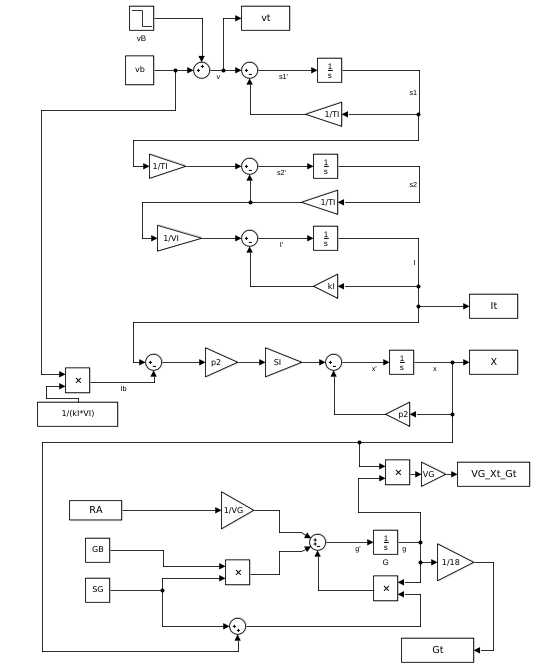
\includegraphics[width=0.9\columnwidth]{bmm.png} 
	\caption{Schéma Bergmanovho minimálneho modelu s podsystémom vstrebávania inzulínu.}
	\label{fig:bmm}
\end{figure}

\begin{figure}
	\centering
	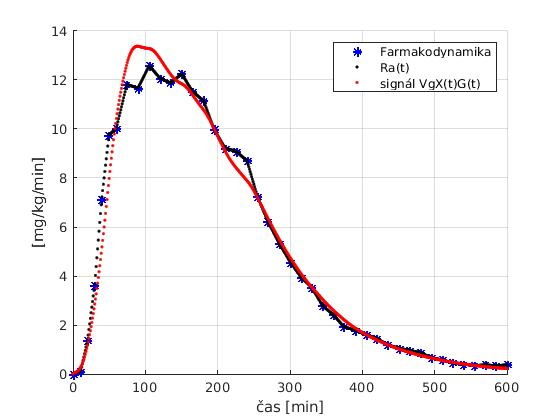
\includegraphics[width=0.7\columnwidth]{toky_glukozy_vzorova.jpg} 
	\caption{Toky glukózy.}
	\label{fig:toky_glukozy}
\end{figure}

\begin{figure}
	\centering
	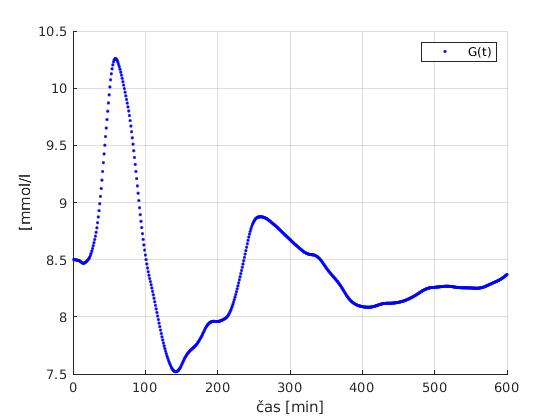
\includegraphics[width=0.7\columnwidth]{glykemia_vzorova.jpg} 
	\caption{Priebeh hladiny glykémie.}
	\label{fig:hladina_glykemie}
\end{figure}

\vspace{10mm}

\subsection{Identifikácia parametrov} \label{subsec:ids2}

Parametre na identifikáciu:
\begin{itemize}
\item $S_I$ $[min]$
\item $p_2$ $[l/min]$ 
\end{itemize}

Pri identifikácií sme sa rozhodli použiť znova genetický algoritmus, ktorý sme nastavili podobným spôsobom ako bolo popísané v časti 1.4,
takže sme sa opať snažili o stredne vysoký selektívny tlak a stredne vysokú diverzitu (5\% najlepších, 20\% mutácie), v tomto prípade sa chromozón skladal iba z dvoch častí $p2$ a $S_I$ a iniciálnu populáciu jedincov sme vygenerovali s týmito ohraničeniami, ktoré sme identifikovali experimentálne: 
\[ 0.0001 < p_2 < 0.1, \hspace{3mm} 0.0001 < S_I < 0.1 \] 
a účelovú funkciu sme volili vo forme:

\begin{equation}
 min \hspace{5mm} \| G_b - \hat{y}(\theta_2) \|^2 + \sum( max(0, G_b - \hat{y}(\theta_2) ))
\end{equation} 

rovnako ako v učebnom texte, 

Pri tejto identifikácií použijeme nami identifikované predchádzajúcej simulácie použijeme:
\begin{itemize}
\item $T_I$ = 44,55  $[min]$
\item $k_I$ = 0,1645 $[l/min]$ 
\item $V_I$ = 147,7954 $[dl/kg]$ 
\end{itemize}

S takto nastavenou identifikáciou sme dospeli k nasledujúcim výsledkom: 
\begin{itemize}
\item $S_I$ = 0,0039 $[min]$
\item $p_2$ = 0,0185 $[l/min]$ 
\end{itemize}

\begin{figure}[h] 
	\centering
	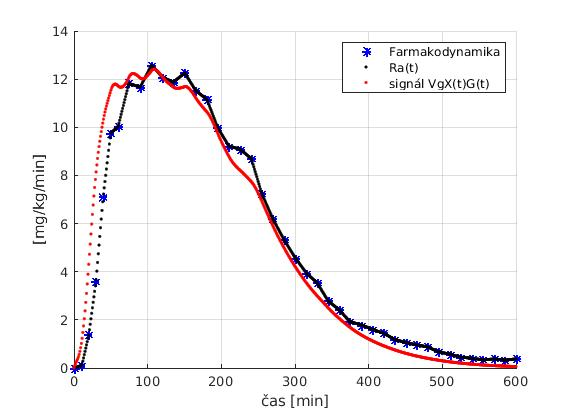
\includegraphics[width=0.5\columnwidth]{toky_glukozy_vlastne.jpg} 
	\caption{Toky glukózy získané identifikovanými parametrami.}
	\label{fig:toky_glukozy}
\end{figure}

\begin{figure}
	\centering
	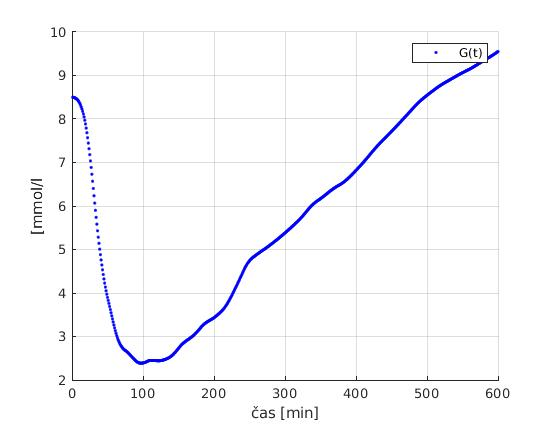
\includegraphics[width=0.5\columnwidth]{glykemia_vlastna.jpg} 
	\caption{Priebeh hladiny glykémie získaný identifikovanými parametrami.}
	\label{fig:hladina_glykemie}
\end{figure}

\vspace{45mm}

\section{Vyhodnotenie výsledkov}

V práci sme sa snažili namodelovať simulátor diabetu, pre prípad, že máme k dispozícií dáta farmakokinetiky a farmakodynamiky, čo by v praxi malo kopírovať situáciu, keď sa priamo do krvi zavedie infúzia glukózy. K tomu bolo potrebné si vytvoriť podsystém pre vstrebávanie inzulínu, ktorý sme vytvárali analogicky s modelovaním Bergmanovho minimálneho modelu a na účely jeho identifikácie sme použili dáta farmakokinetiky. Výstup tohto podsystému sme zaviedli ako jeden zo vstupov do nášho Bergmanovho minimálneho modelu, druhý vstup tvorili dáta farmakodynamiky, ktoré sme dointerpolovali a použili ich ako vstup $Ra(t)$. Takto poskladaný model nám dokáže modelovať zmenu stavu glykémie, vhľadom na načítané dáta farmakodynamiky a nastavené parametre.

Podarilo sa nám dopracovať k parametrom, ktoré zhruba modelujú priebeh glykémie, aj keď sa z toho


%\section{Identifikácia parametrov Bergmanovho modelu}

%\section{Vyhodnotenie výsledkov identifikácie}


%%----------------------------------------------------------------------------------------
%%	EQUATION EXAMPLES
%%----------------------------------------------------------------------------------------
%
%\section{Interpreting Equations}
%
%\subsection{Identify the author of Equation \ref{eq:bayes} below and briefly describe it in English.}
%
%\begin{align} 
%	\label{eq:bayes}
%	\begin{split}
%		P(A|B) = \frac{P(B|A)P(A)}{P(B)}
%	\end{split}					
%\end{align}
%
%Lorem ipsum dolor sit amet, consectetur adipiscing elit. Praesent porttitor arcu luctus, imperdiet urna iaculis, mattis eros. Pellentesque iaculis odio vel nisl ullamcorper, nec faucibus ipsum molestie. Sed dictum nisl non aliquet porttitor. Etiam vulputate arcu dignissim, finibus sem et, viverra nisl. Aenean luctus congue massa, ut laoreet metus ornare in. Nunc fermentum nisi imperdiet lectus tincidunt vestibulum at ac elit. Nulla mattis nisl eu malesuada suscipit.
%
%%------------------------------------------------
%
%\subsection{Try to make sense of some more equations.}
%
%\begin{align} 
%	\begin{split}
%		(x+y)^3 &= (x+y)^2(x+y)\\
%		&=(x^2+2xy+y^2)(x+y)\\
%		&=(x^3+2x^2y+xy^2) + (x^2y+2xy^2+y^3)\\
%		&=x^3+3x^2y+3xy^2+y^3
%	\end{split}					
%\end{align}
%
%Lorem ipsum dolor sit amet, consectetuer adipiscing elit. 
%\begin{align}
%	A = 
%	\begin{bmatrix}
%		A_{11} & A_{21} \\
%		A_{21} & A_{22}
%	\end{bmatrix}
%\end{align}
%Aenean commodo ligula eget dolor. Aenean massa. Cum sociis natoque penatibus et magnis dis parturient montes, nascetur ridiculus mus. Donec quam felis, ultricies nec, pellentesque eu, pretium quis, sem.
%
%%----------------------------------------------------------------------------------------
%%	LIST EXAMPLES
%%----------------------------------------------------------------------------------------
%
%\section{Viewing Lists}
%
%\subsection{Bullet Point List}
%
%\begin{itemize}
%	\item First item in a list 
%		\begin{itemize}
%		\item First item in a list 
%			\begin{itemize}
%			\item First item in a list 
%			\item Second item in a list 
%			\end{itemize}
%		\item Second item in a list 
%		\end{itemize}
%	\item Second item in a list 
%\end{itemize}
%
%%------------------------------------------------
%
%\subsection{Numbered List}
%
%\begin{enumerate}
%	\item First item in a list 
%	\item Second item in a list 
%	\item Third item in a list
%\end{enumerate}
%
%%----------------------------------------------------------------------------------------
%%	TABLE EXAMPLE
%%----------------------------------------------------------------------------------------
%
%\section{Interpreting a Table}
%
%\begin{table}[h] % [h] forces the table to be output where it is defined in the code (it suppresses floating)
%	\centering % Centre the table
%	\begin{tabular}{l l l}
%		\toprule
%		\textit{Per 50g} & \textbf{Pork} & \textbf{Soy} \\
%		\midrule
%		Energy & 760kJ & 538kJ\\
%		Protein & 7.0g & 9.3g\\
%		Carbohydrate & 0.0g & 4.9g\\
%		Fat & 16.8g & 9.1g\\
%		Sodium & 0.4g & 0.4g\\
%		Fibre & 0.0g & 1.4g\\
%		\bottomrule
%	\end{tabular}
%	\caption{Sausage nutrition.}
%\end{table}
%
%%------------------------------------------------
%
%\subsection{The table above shows the nutritional consistencies of two sausage types. Explain their relative differences given what you know about daily adult nutritional recommendations.}
%
%Lorem ipsum dolor sit amet, consectetur adipiscing elit. Praesent porttitor arcu luctus, imperdiet urna iaculis, mattis eros. Pellentesque iaculis odio vel nisl ullamcorper, nec faucibus ipsum molestie. Sed dictum nisl non aliquet porttitor. Etiam vulputate arcu dignissim, finibus sem et, viverra nisl. Aenean luctus congue massa, ut laoreet metus ornare in. Nunc fermentum nisi imperdiet lectus tincidunt vestibulum at ac elit. Nulla mattis nisl eu malesuada suscipit.
%
%%----------------------------------------------------------------------------------------
%%	CODE LISTING EXAMPLE
%%----------------------------------------------------------------------------------------
%
%\section{Reading a Code Listing}
%
%\lstinputlisting[
%	caption=Luftballons Perl Script., % Caption above the listing
%	label=lst:luftballons, % Label for referencing this listing
%	language=Perl, % Use Perl functions/syntax highlighting
%	frame=single, % Frame around the code listing
%	showstringspaces=false, % Don't put marks in string spaces
%	numbers=left, % Line numbers on left
%	numberstyle=\tiny, % Line numbers styling
%	]{luftballons.pl}
%
%%------------------------------------------------
%
%\subsection{How many luftballons will be output by the Listing \ref{lst:luftballons} above?}
%
%Aliquam arcu turpis, ultrices sed luctus ac, vehicula id metus. Morbi eu feugiat velit, et tempus augue. Proin ac mattis tortor. Donec tincidunt, ante rhoncus luctus semper, arcu lorem lobortis justo, nec convallis ante quam quis lectus. Aenean tincidunt sodales massa, et hendrerit tellus mattis ac. Sed non pretium nibh. Donec cursus maximus luctus. Vivamus lobortis eros et massa porta porttitor.

%------------------------------------------------

%\subsection{Identify the regular expression in Listing \ref{lst:luftballons} and explain how it relates to the anti-war sentiments found in the rest of the script.}
%
%Fusce varius orci ac magna dapibus porttitor. In tempor leo a neque bibendum sollicitudin. Nulla pretium fermentum nisi, eget sodales magna facilisis eu. Praesent aliquet nulla ut bibendum lacinia. Donec vel mauris vulputate, commodo ligula ut, egestas orci. Suspendisse commodo odio sed hendrerit lobortis. Donec finibus eros erat, vel ornare enim mattis et.

%----------------------------------------------------------------------------------------

\end{document}
